\begin{figure}[t]
    \centering
   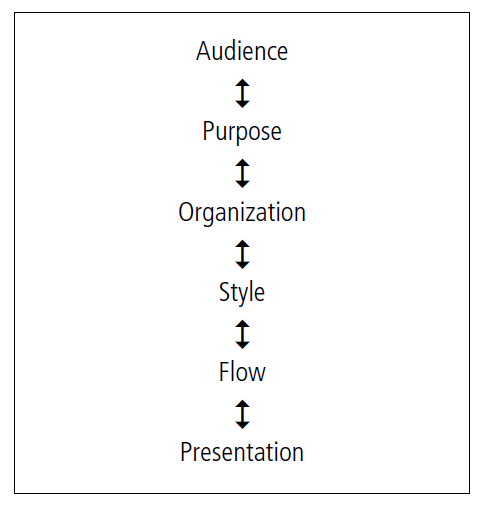
\includegraphics[width=0.5\textwidth]{figures/research/writing_considerations.PNG}
    \caption{Considerations in Academic Writing~\cite{Swales2012}}
    \label{fig:writing_considerations}
\end{figure}

According to~\citeauthor{Swales2012}, academic writing is a product of many considerations which can be categorized in five units: audience, purpose, organization, style, flow, and presentation (see Figure \ref{fig:writing_considerations}).
Audience and purpose are typically interconnected. The first consideration towards a successful writing is to identify the audience. 
For most students, the audience will be a tutor presumably knowledgeable about the writing topic. 
Other possible audiences include external experts (i.e. partners in education) and graduation committees (i.e. those who will review and assess graduation dissertations, usually university staff and external experts). 
Understanding the audience will better define a writer's purpose and strategy (or strategies). If the audience knows less than the writer, the writer’s purpose is often instructional (as in a manual). 
If the audience knows more than the writer, the writer’s purpose is usually to display familiarity, expertise, and intelligence. The latter is a common situation for the undergraduate student writer.
\\\\
Academic writing has also expected patterns of organizing the information for a particular type of text. 
A type of text is referred to as general-specific, which can be used to produce an introduction paragraph or definitions. 
As the name suggests, these texts involve moving from broader statements to more specific ones. 
The opposite of general-specific is specific-to-general texts, which can structure conclusions and recommendations. 
An important text pattern is the problem-to-solution, especially since academic research focuses on solving problems. 
A problem-to-solution structured text is usually presenting the situation, reasons the problem, discusses ways to alleviate the problem and then evaluates proposed solution(s).
However, often an incomplete solution is offered which may introduce a new problem that will then be addressed similarly. 
Other ways of organizing text enumerate comparison-contrast, cause-effect and classification~\cite{Swales2012}.
\\\\
One difficulty of undergraduate student writers in using the appropriate style. 
Most aiding tools and programs are written primarily to find spelling and basic grammar errors, not to offer stylistic advice for academic writing.
While  stylistic conventions differ in every field, most common stylistic conventions in the field of \acrshort{ict} enumerate: passive voice, addressing the reader (i.e. You can see the results in Table 1), contractions (i.e. don't, isn't), language that softens a point (i.e. may, appears to), concise sentences (i.e. nominalization).
\\\\
Another important consideration for successful communication is flow: moving from one statement in a text to the next. Naturally, establishing a clear connection of ideas is important to help the reader follow the text. 
Although most writers' first instinct is to use logical connectors (i.e. however or furthermore), following a progression from old or given information to new information is generally preferred
Placing relevant 'old' information in early position establishes a content connection backward and provides a forward content link that establishes the context. 
Furthermore, logical connectors rise the issue of punctuation.
Many general style guides and style guides are specific to a  field of study, however, most common punctuation enumerate: semicolons (;), colons (:), dashes (—), and commas (,).
\\\\
Finally, and most importantly, the presentation of a writing task is key in academic writing.
Most instructors tolerate small errors in language in papers written by nonnative speakers—for example, mistakes in article or preposition usage. 
However, errors that instructors think could have been avoided by careful proofreading are generally considered less acceptable.
Thus, an instructor's focus should be more on content and information flow first rather then grammar or text formatting.
\\\\
\textit{Writing research}
\\\\
Research governs academic writing. 
While there are different types of research as well as different types of research writing, several text formatting aspects are expected in an academic research writing.
The content generally follows the standard Introduction-Method-Result-Discussion (IMRD) pattern. 
As shown in Figure \ref{fig:research_writing_formatting}, the arrows indicate that the sections are closely connected, moving from generals-specific to specific-to-general information.
The main purpose of the Introduction is to provide the rationale for the research, moving from a general discussion of the topic to the particular question, issue, or hypothesis being investigated. but also to attract interest in the topic-and hence readers.
The Methods section describes, in various degrees of detail, methodology and materials, while in the Results section, the findings are described, accompanied by variable amounts of commentary.
The Discussion section gives meaning to and interprets the results in a variety of ways, referring to statements made in the Introduction.
Furthermore, most frequent writing considerations encountered in IMRD are shown in Table \ref{table:frequent_writing_considerations}.

\begin{figure}[t]
    \centering
   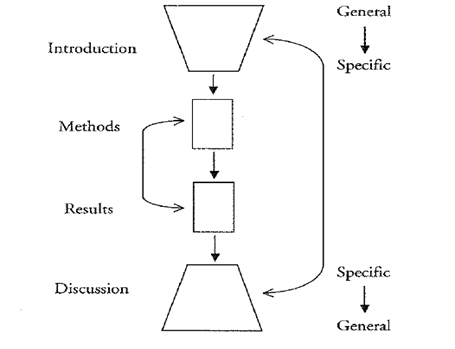
\includegraphics[width=0.65\textwidth]{figures/research/research_writing_formatting.png}
    \caption{Overall Research Writing Structure~\cite{Swales2012}}
    \label{fig:research_writing_formatting}
\end{figure}

\begin{table*}[t]
\centering
\caption{Frequent Academic Writing Considerations}
\begin{tabular}{|l|l|l|l|l|}
 \hline
     & \textbf{Introduction} & \textbf{Methods} & \textbf{Results} & \textbf{Discussion} \\
 \hline
    Present tense & high & low & low & high \\
 \hline 
    Past tense & mid & high & high & mid \\
 \hline
    Present perfect & mid & low & low & mid \\
 \hline 
    Passive & low & high & variable & variable \\
 \hline
    Citations & mid & mid & variable & mid \\
 \hline
    Hedging & mid & low & mid & high \\
 \hline
\end{tabular}
\label{table:frequent_writing_considerations}
\end{table*}
